\documentclass[a4paper,11pt]{report}
\usepackage{chuan_math_gkt}
\usetikzlibrary{angles,quotes,intersections,patterns,decorations.pathreplacing}
\chuanexamsetup

\begin{document}
\examfontsize

\examsecret{绝密$\bigstar$启用前}

\examtitle{2021年普通高等学校招生全国统一考试（全国甲卷文科）}{数\quad 学}

\noticetitle
\begin{examnotice}
\item 答卷前，考生务必将自己的姓名、准考证号填写在答题卡上. 
\item 回答选择题时，选出每小题的答案后，用铅笔把答题卡上对应题目的答案标号涂黑. 如需改动，用橡皮擦干净后，再选涂其他答案标号. 回答非选择题时，将答案写在答题卡上. 写在本试卷上无效. 
\item 考试结束后，将本试卷和答题卡一并交回. 
\end{examnotice}

\examsection{一、选择题：本题共12小题，每小题5分，共60分. 在每小题给出的四个选项中，只有一项是符合题目要求的.}
\begin{examquestions}

\item 设集合 $M=\{1,3,5,7,9\}$，$N=\{x\mid 2x>7\}$，则 $M\cap N=$
\fourchoices{$\{7,9\}$}{$\{5,7,9\}$}{$\{3,5,7,9\}$}{$\{1,3,5,7,9\}$}

\item 为了解某地农村经济情况，对该地农户家庭年收入进行抽样调查，将农户家庭年收入的调查数据整理得到如下频率分布直方图：

\begin{tightcenter}
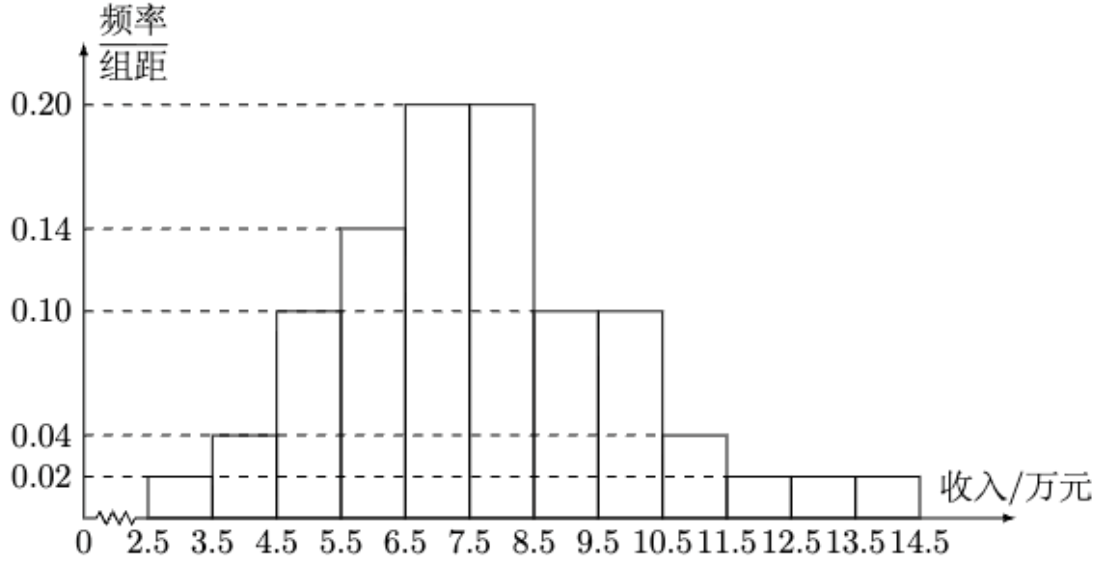
\includegraphics[width=9cm]{figures/2021_jia_li_image8.png}
\end{tightcenter}

根据此频率分布直方图，下面结论中不正确的是
\onechoices
{该地农户家庭年收入低于 $4.5$ 万元的农户比率估计为 $6\%$}
{该地农户家庭年收入不低于 $10.5$ 万元的农户比率估计为 $10\%$}
{估计该地农户家庭年收入平均值不超过 $6.5$ 万元}
{估计该地有一半以上的农户，其家庭年收入介于 $4.5$ 万元至 $8.5$ 万元之间}

\item 已知 $(1-\mathrm{i})^2z=3+2\mathrm{i}$，则 $z=$
\fourchoices
{\tallchoice{$-1-\dfrac32\mathrm{i}$}}
{\tallchoice{$-1+\dfrac32\mathrm{i}$}}
{\tallchoice{$-\dfrac32+\mathrm{i}$}}
{\tallchoice{$-\dfrac32-\mathrm{i}$}}

\item 下列函数中是增函数的为
\fourchoices
{$f(x)=-x$}
{\tallchoice{$f(x)=\left(\dfrac23\right)^x$}}
{$f(x)=x^2$}
{$f(x)=\sqrt[x]{3}$}

\item 点 $(3,0)$ 到双曲线 $\dfrac{x^2}{16}-\dfrac{y^2}{9}=1$ 一条渐近线的距离为
\fourchoices
{\tallchoice{$\dfrac95$}}
{\tallchoice{$\dfrac85$}}
{\tallchoice{$\dfrac65$}}
{\tallchoice{$\dfrac45$}}

\item 青少年视力是社会普遍关注的问题，视力情况可借助视力表测量. 通常用五分记录法和小数记录法记录视力数据，五分记录法的数据 $L$ 和小数记录表的数据 $V$ 满足 $L=5+\lg V$. 已知某同学视力的五分记录法的数据为 $4.9$，则其视力的小数记录法的数据为（$\sqrt[10]{10}\approx1.259$）
\fourchoices{$1.5$}{$1.2$}{$0.8$}{$0.6$}

\item 在一个正方体中，过顶点 $A$ 的三条棱的中点分别为 $E,F,G$. 该正方体截去三棱锥 $A-EFG$ 后，所得多面体的三视图中，正视图如图所示，则相应的侧视图是

\begin{tightcenter}
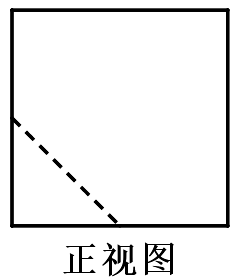
\includegraphics[width=2cm]{figures/2021_jia_wen_image29.png}
\end{tightcenter}

\graphchoicesoneline
{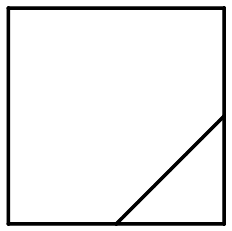
\includegraphics[width=2cm]{figures/2021_jia_wen_image30.png}}
{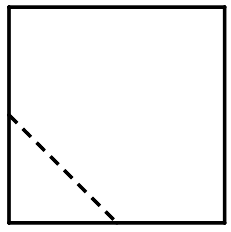
\includegraphics[width=2cm]{figures/2021_jia_wen_image31.png}}
{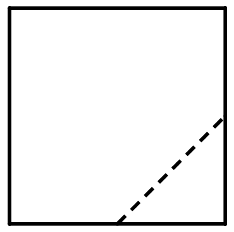
\includegraphics[width=2cm]{figures/2021_jia_wen_image32.png}}
{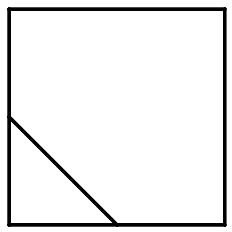
\includegraphics[width=2cm]{figures/2021_jia_wen_image33.png}}

\item 在 $\triangle ABC$ 中，已知 $B=120^\circ$，$AC=\sqrt{19}$，$AB=2$，则 $BC=$
\fourchoices{$1$}{$\sqrt2$}{$\sqrt5$}{$3$}

\item 记 $S_n$ 为等比数列 $\{a_n\}$ 前 $n$ 项和. 若 $S_2=4$，$S_4=6$，则 $S_6=$
\fourchoices{$7$}{$8$}{$9$}{$10$}

\item 将 $3$ 个 $1$ 和 $2$ 个 $0$ 随机排成一行，则 $2$ 个 $0$ 不相邻的概率为
\fourchoices{$0.3$}{$0.5$}{$0.6$}{$0.8$}

\item 若 $\alpha\in\left(0,\dfrac{\pi}{2}\right)$，$\tan2\alpha=\dfrac{\cos\alpha}{2-\sin\alpha}$，则 $\tan\alpha=$
\fourchoices
{\tallchoice{$\dfrac{\sqrt{15}}{15}$}}
{\tallchoice{$\dfrac{\sqrt5}{5}$}}
{\tallchoice{$\dfrac{\sqrt5}{3}$}}
{\tallchoice{$\dfrac{\sqrt{15}}{3}$}}

\item 设 $f(x)$ 是定义域为 $\mathbb R$ 的奇函数，且 $f(1+x)=f(-x)$. 若 $f\left(-\dfrac13\right)=\dfrac13$，则 $f\left(\dfrac53\right)=$
\fourchoices
{\tallchoice{$-\dfrac53$}}
{\tallchoice{$-\dfrac13$}}
{\tallchoice{$\dfrac13$}}
{\tallchoice{$\dfrac53$}}

\end{examquestions}

\examsection{二、填空题：本题共4小题，每小题5分，共20分.}
\begin{examquestions}[start=13]

\item 若向量 $\vec a,\vec b$ 满足 $|\vec a|=3$，$|\vec a-\vec b|=5$，$\vec a\cdot\vec b=1$，则 $|\vec b|=$ \blank.

\item 已知一个圆锥的底面半径为 $6$，其体积为 $30\pi$，则该圆锥的侧面积为 \blank.

\item 已知函数 $f(x)=2\cos(\omega x+\varphi)$ 的部分图像如图所示，则 $f\left(\dfrac{\pi}{2}\right)=$ \blank.

\begin{tightcenter}
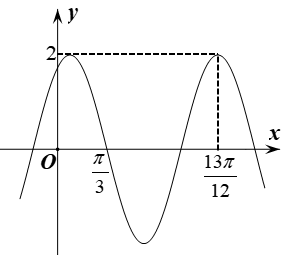
\includegraphics[width=5cm]{figures/2021_jia_wen_image66.png}
\end{tightcenter}

\item 已知 $F_1,F_2$ 为椭圆 $C:\dfrac{x^2}{16}+\dfrac{y^2}{4}=1$ 的两个焦点，$P,Q$ 为 $C$ 上关于坐标原点对称的两点，且 $|PQ|=|F_1F_2|$，则四边形 $PF_1QF_2$ 的面积为 \blank.

\end{examquestions}

\examsection{三、解答题：共70分. 解答应写出文字说明、证明过程或演算步骤. 第17题～第21题为必考题，每个试题考生都必须作答. 第22、23题为选考题，考生根据要求作答.}
\begin{examanswers}[start=17]

\item（12分）

甲、乙两台机床生产同种产品，产品按质量分为一级品和二级品，为了比较两台机床产品的质量，分别用两台机床各生产了 $200$ 件产品，产品的质量情况统计如下表：

\begin{tightcenter}
{\renewcommand{\arraystretch}{0.9}
\begin{tabular}{|c|c|c|c|}
\hline
& 一级品 & 二级品 & 合计 \\ \hline
甲机床 & $150$ & $50$ & $200$ \\ \hline
乙机床 & $120$ & $80$ & $200$ \\ \hline
合计 & $270$ & $130$ & $400$ \\ \hline
\end{tabular}}
\end{tightcenter}

\subq{（1）}{甲机床、乙机床生产的产品中一级品的频率分别是多少？}

\subq{（2）}{能否有 $99\%$ 把握认为甲机床的产品质量与乙机床的产品质量有差异？
附：$K^2=\dfrac{n(ad-bc)^2}{(a+b)(c+d)(a+c)(b+d)}$

\begin{tightcenter}
{\renewcommand{\arraystretch}{0.9}
\begin{tabular}{|c|c|c|c|}
\hline
$P(K^2\geq k)$ & $0.050$ & $0.010$ & $0.001$ \\ \hline
$k$ & $3.841$ & $6.635$ & $10.828$ \\ \hline
\end{tabular}}
\end{tightcenter}
}

\item（12分）

记 $S_n$ 为数列 $\{a_n\}$ 的前 $n$ 项和，已知 $a_n>0$，$a_2=3a_1$，且数列 $\{\sqrt{S_n}\}$ 是等差数列，证明：$\{a_n\}$ 是等差数列.

\item（12分）

已知直三棱柱 $ABC-A_1B_1C_1$ 中，侧面 $AA_1B_1B$ 为正方形，$AB=BC=2$，$E,F$ 分别为 $AC$ 和 $CC_1$ 的中点，$BF\perp A_1B_1$.

\noindent\begin{minipage}[t]{0.65\linewidth}
\subq{（1）}{求三棱锥 $F-EBC$ 的体积；}

\subq{（2）}{已知 $D$ 为棱 $A_1B_1$ 上的点，证明：$BF\perp DE$.}
\end{minipage}\hfill
\begin{minipage}[t]{0.26\linewidth}
\vspace{-2em}
\centering
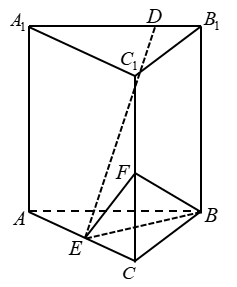
\includegraphics[width=\linewidth]{figures/2021_jia_wen_image81.png}
\end{minipage}

\vspace{-3.5em}

\item（12分）

设函数 $f(x)=a^2x^2+ax-3\ln x+1$，其中 $a>0$.

\subq{（1）}{讨论 $f(x)$ 的单调性；}

\subq{（2）}{若 $y=f(x)$ 的图象与 $x$ 轴没有公共点，求 $a$ 的取值范围.}

\item（12分）

抛物线 $C$ 的顶点为坐标原点 $O$. 焦点在 $x$ 轴上，直线 $l:x=1$ 交 $C$ 于 $P,Q$ 两点，且 $OP\perp OQ$. 已知点 $M(2,0)$，且 $\odot M$ 与 $l$ 相切.

\subq{（1）}{求 $C$，$\odot M$ 的方程；}

\subq{（2）}{设 $A_1,A_2,A_3$ 是 $C$ 上的三个点，直线 $A_1A_2$，$A_1A_3$ 均与 $\odot M$ 相切. 判断直线 $A_2A_3$ 与 $\odot M$ 的位置关系，并说明理由.}

\item（10分）【选修4-4：坐标系与参数方程】

在直角坐标系 $xOy$ 中，以坐标原点为极点，$x$ 轴正半轴为极轴建立极坐标系，曲线 $C$ 的极坐标方程为 $\rho=2\sqrt2\cos\theta$.

\subq{（1）}{将 $C$ 的极坐标方程化为直角坐标方程；}

\subq{（2）}{设点 $A$ 的直角坐标为 $(1,0)$，$M$ 为 $C$ 上的动点，点 $P$ 满足 $\vec{AP}=\sqrt2\vec{AM}$，写出 $P$ 的轨迹 $C_1$ 的参数方程，并判断 $C$ 与 $C_1$ 是否有公共点.}

\item（10分）【选修4-5：不等式选讲】

已知函数 $f(x)=|x-2|$，$g(x)=|2x+3|-|2x-1|$.

\noindent\begin{minipage}[t]{0.65\linewidth}

\subq{（1）}{画出 $y=f(x)$ 和 $y=g(x)$ 的图像；}

\subq{（2）}{若 $f(x+a)\geq g(x)$，求 $a$ 的取值范围.}
\end{minipage}\hfill
\begin{minipage}[t]{0.26\linewidth}
\vspace{-3em}
\centering
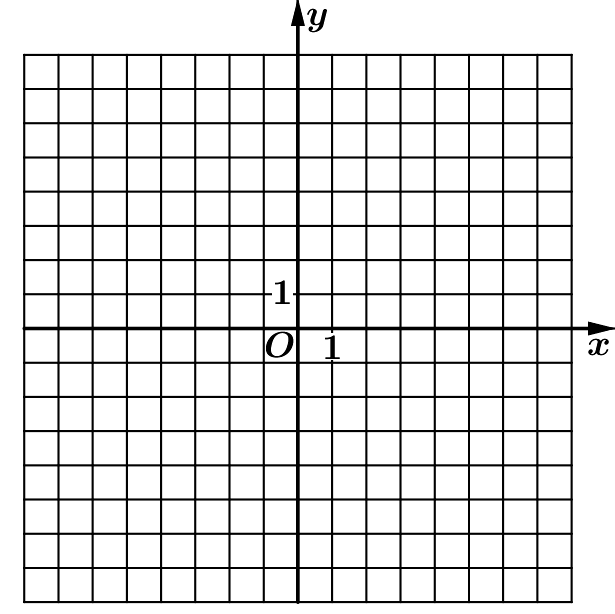
\includegraphics[width=\linewidth]{figures/2021_jia_wen_image103.png}
\end{minipage}




\end{examanswers}

\end{document}